\subsection{A Neural Probabilistic Language Model \cite{Bengio2003A}}

This paper proposes a neural network architecture to learn a probabilistic language model. The method can simultaneously learn a distributed representation for each word and the probability function for word sequences.

A goal of statistical language modeling is to learn the joint probability function of sequences of words in a language. It can be represented by the conditional probability of the next word given all the previous ones:
$$P(w_1^T) = \prod_{i=1}^T P(w_t | w_1^{t-1}).$$
Here $w_t$ is  the $t$-th word, and $w_i^j = (w_i, w_{i+1},... , w_j)$ is the subsequence from the $i$-th to the $j$-th word.

One of the motivations of this paper is that traditional $n$-gram models do not take into account of the similarity between words. For example, having seen the sentence ``The cat is walking in the bedroom'' in the training corpus, a model should assign high probability to the sentence ``A dog was running in a room'', because ``the'' and ``a'', ``dog'' and ``cat'' are similar to each other.

The basic idea of the proposed approach can be summarized as follows: 1) Associate with each word a distributed word feature vector (a real-valued vector in $\mathbb{R}^m$); 2) Express the joint probability function of word sequences in terms of the feature vectors; 3) Learn simultaneously the word feature vectors and the probability function.

Specifically, the objective of the neural network is to learn a good model $f(w_t, ..., w_{t-n+1}) = P(w_t | w_1^{t-1})$. The function $f(w_t, ..., w_{t-n+1})$ is decomposed in two parts:

\begin{enumerate}
\item A mapping $C$ from any element $i$ from the vocabulary $V$ to a real vector $C(i) \in \mathbb{R}^m$. It represents the distributed feature vectors associated with each word.
\item The probability function over words, which is denoted by $g$. The input of $g$ is a sequence of feature vectors of words in context ($C(w_{t-n+1}),..., C(w_{t-1})$), and the output is a vector whose $i$-th element estimates the probability of next word being $i$ ($P(w_t = i | w_1^{t-1})$).
\end{enumerate}

\begin{figure}[htbp]
  \centering
  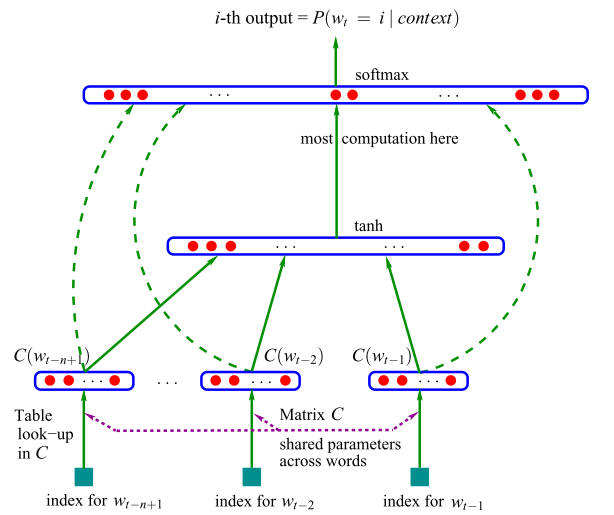
\includegraphics[width=.8\linewidth]{8_15_DL}\\
  \caption{An overview of the network architecture}\label{fig:DL}
\end{figure}

Figure \ref{fig:DL} shows the proposed neural architecture. The objective  function $f$ is a composition of $C$ and $g$, with $C$ being shared across all the words in the context. The function $g$ can be implemented by a feed-forward or recurrent neural network. This paper uses the ordinary hyperbolic tangent hidden layer with a softmax output layer.

The paper also explores parallelization on two types of platforms: shared-memory processor machines and Linux clusters with a fast network. In the case of a shared-memory processor, each processor works on a different subset of the data. Each processor computes the gradient for its examples, and performs stochastic gradient updates on the parameters of the model, which are simply stored in a shared-memory area. If the parallel computer is a network of CPUs, the paper chooses to parallelize across the parameters of the output units. The CPUs need to communicate the normalization factor of the output softmax, and the gradients on the hidden layer with the word feature layer. All the CPUs will duplicate the computations that precede the output units. After this step, each processor works on its local data as before.

In this experimental section, the paper measures the perplexity of the proposed model, and compares the results with several previous work. It is reported that the proposed method outperforms the most competitive alternative approach by up to 24\% in perplexity. 